% TEMPLATE for Usenix papers, specifically to meet requirements of
%  USENIX '05
% originally a template for producing IEEE-format articles using LaTeX.
%   written by Matthew Ward, CS Department, Worcester Polytechnic Institute.
% adapted by David Beazley for his excellent SWIG paper in Proceedings,
%   Tcl 96
% turned into a smartass generic template by De Clarke, with thanks to
%   both the above pioneers
% use at your own risk.  Complaints to /dev/null.
% make it two column with no page numbering, default is 10 point

% Munged by Fred Douglis <douglis@research.att.com> 10/97 to separate
% the .sty file from the LaTeX source template, so that people can
% more easily include the .sty file into an existing document.  Also
% changed to more closely follow the style guidelines as represented
% by the Word sample file. 

% Note that since 2010, USENIX does not require endnotes. If you want
% foot of page notes, don't include the endnotes package in the 
% usepackage command, below.

% This version uses the latex2e styles, not the very ancient 2.09 stuff.

% Updated July 2018: Text block size changed from 6.5" to 7"

\documentclass[letterpaper,twocolumn,10pt]{article}
\usepackage{usenix2019,epsfig,endnotes,algpseudocode,algorithm}
\begin{document}

%don't want date printed
\date{}

% make title bold and 14 pt font (Latex default is non-bold, 16 pt)
% we shouldn't say these are internet connected because some aren't
\title{\Large \bf Hacking Electronic Bike Shifters with Wireless Functionality }

%for single author (just remove % characters)
\author{
  {\rm Thomas Hansen}\\
  UW Madison
  \and
  {\rm Tolga Beser}\\
  UW Madison
  \and
  {\rm Chang-Yen Tseng}\\
  UW Madison
  % copy the following lines to add more authors
  % \and
  % {\rm Name}\\
  %Name Institution
} % end author

\maketitle

% Use the following at camera-ready time to suppress page numbers.
% Comment it out when you first submit the paper for review.
\thispagestyle{empty}


%-------------------------------------------------------------------------------
\begin{abstract}
  %-------------------------------------------------------------------------------
  Electronic shifters have become increasingly accessible for professional and casual riders, but they bring new security threats and technical challenges. Riders own safety depend on their bikes and they need to perform at their best. Because of their importance, we decided to take 3 shifters, each with a different wireless configuration, and test them against a variety of wireless attacks attempting to manipulate the bikes behavior without the riders consent, either to hurt their performance in a race, strand the user, or force them to crash.

  We limited ourselves to wireless attacks and studied the components design to try and find attacks that would work best. We found the SRAM groupset was vulnerable to replay attacks, and the Archer Components allowed unverified users to connect to the device. The Shimano Di2 system which relies on wired shifting appeared to be the most secure, as it's the only system with a password which requires you to restart the device if you enter the password incorrectly. This would require brute force attacks to have access to the physical device and take a long time, even for technically advanced users.
\end{abstract}

% alternate option, left-alights title without giving it a number
% \subsection*{Abstract}

\section{Introduction}

% A paragraph of text goes here.  Lots of text.  Plenty of interesting text. \\

% More fascinating text. Features\endnote{Remember to use endnotes, not footnotes!} galore, plethora of promises.\\

Cycling has seen the emergence of electronic shifting technologies over the past few years. While the technology existed as far back as the 1990s, adoption has accelerated, especially for high-end bikes. As we see the technology improve, these shifters have become faster and more precise than mechanical shifting, allowing users to shift more quickly, shift standing, and prevent chain rub. Every major brand has introduced their own line of electronic shifters including Shimano, SRAM, Campagnolo, as well as smaller brands such as Archer.

The wireless shifters use an assortment of communication technologies known as Personal Area Networks (PAN’s) such as Bluetooth. The use of these technologies opens the once closed off bicycle to security vulnerabilities. If an attacker can trigger extraneous shifts the cyclist can be thrown off their bike causing personal injury and the potential for even larger accidents (cyclists in pro races are tightly packed causing crashes to spread quickly). While security research focused on these electronic shifters is sparse there exists a plethora of work exploring security for various Personal Area Network enabled devices. A subset of wireless shifters utilizes Bluetooth as a communication protocol which has been shown to have security flaws in several implementations~ \cite{JiWu}. One of the wireless shifting devices that we would like to examine is the SRAM eTAP system which utilizes their own novel Airea Personal Area Network protocol which allows their components to communicate from up to a hundred meters away. This large distance could allow an attacker to communicate with their components from an unobservable location.

\section{Related Work}

There has been a lot of work into researching how to break wireless networks on embedded electronic devices, especially those where security was not an upfront concern. Many simply use replay attacks and exploit design flaws with device authentication~ \cite{Halperin}. Other papers look broadly on the state of wireless security, and analyse methods surrounding IoT devices and wireless communication methods~\cite{Choi}~\cite{Radek}.

We attempted to take many of these findings and bring them to the electronic shifting space to see what sorts of vulnerabilities we could find. To the best of our knowledge, there is no comprehensive research on the security of wireless bike shifters. We studied the Archer Components D1X, SRAM eTap, and Shimano Di2 for vulnerabilities.

\section{Potential Impact}

Electronic shifters in bikes have become extremely popular among high-end bikes. Tadej Pogačar, the overall winner of the 2020 and 2021 tour won using a Campagnolo EPS shifter. Egan Bernal, the 2019 winner, won riding a Pinarello that used Shimano Dura Ace Di2 shifters~ \cite{GCNTech}. Furthermore, high-end bikes such as the Trek Madone 9 recommend electronic shifters.

Competitions also raise the stakes for the potential impact exploits may have. The Tour de France prize pool is 3.6 million AU, and many millions stand to be gained from partnerships and sponsors. Anyone who's able to impact a race in their favor may realize substantial financial gain, and we only expect the potential professional impacts to increase with time.

Casual cyclists are also impacted. Cycling is a sport where casual riders can go out for multi hour rides, and if their bike is disabled or their gears are changed unexpectedly a serious threat may be posed to their wellbeing, stranding them or causing them to crash. Because of these reasons we think the security of electronic shifters is an important topic that deserves research.

\subsection{Contributions}

In summary, our contributions to the field include analyzing the security landscape of wireless bike shifters according to our threat models, and providing recommendations to manufacturers moving forward. We found the SRAM shifter was susceptible to simple replay attacks, while the Archer Bluetooth authentication protocol was left completely open. Lastly we found Shimano was the most secure, rebuffing our attempts to break into it.

\subsection{Common Attacks Against IoT Devices}

Due to the nature of wireless IoT devices and their power limitations potential security flaws have been a concern for years~ \cite{HeXu}. Because the research body is so vast we will derive a few common attack vectors that we believe are most applicable to our study. The attack vectors that we will outline are Replay, Denial of Service, and Man in the Middle Attacks.

\begin{itemize}
  \item \textbf{Replay Attacks} are conducted by recording communication signals between IoT Devices and replaying them. Usually defended against using some session key implementation, these false signals will be non-discernible from the legitimate commands.
  \item \textbf{Denial of Service (DoS)} attacks are effective against most wireless IoT devices. A lack of processing power and battery life often compounds these problems and may allow for a variety of new attacks, even including draining battery life of critical bike components~\cite{Moyers}.
  \item \textbf{Packet Spoofing} are similar to replay attacks however instead of sending the packet out as is the attacker retains the packet and modifies it. This can be used to increment counters, make commands the victim hasn't made yet, or attempt to force the device to perform undefined behavior. A high quality ecryption algorithm can make it hard to spoof packets.
\end{itemize}

\subsection{Research in wireless attacks against other vehicles}

The ushering in of new technology to bicycles is reminiscent of the automotive industries push towards intelligent systems. These changes, however, come with security issues which were highlighted when Chrysler recalled 1.4 million vehicles due to a remote hacking vulnerability that let adversaries control the vehicle and even cut the brakes~\cite{ChryslerRecall}. Remote vehicle hacking has been demonstrated across multiple manufacturers (Tesla, BMW, Chrysler) ~\cite{Tesla}~\cite{BMW}~\cite{Chrysler} and research into the security of such systems is now commonplace~\cite{dibaei2019overview}. Systems utilized by intelligent vehicles such as vehicular ad hoc networks~\cite{SAKIZ201733} (VAHN)enabling vehicle to vehicle communication have been studied and found to pose security risks~\cite{ SAKIZ201733}. With the rise of intelligent/wireless bicycle components the need to assess a security landscape of such components becomes paramount as seen by the changes in the automotive industry.

% \section{Threat Model}

\section{Devices}
\subsection{Archer Components D1X}

The Archer D1X~\cite{Archer} is a modular electronic shifting system that can be integrated into a wide array of derailleur-shifting groupsets. While the other two components groups that we study come with custom derailleurs that are wirelessly enabled, the D1X focuses on integrating into existing systems. It is installed near the derailleur with the shifting cables routing through it. This allows the D1X to change the tensions of the shifting cables and trigger gear changes. The electronic shifting box is connected to the hand shifters through Bluetooth allowing the user to send shifting signals. Of note, the D1X is the only component that we will study that utilizes the Bluetooth protocol for communication between the shifter and shifting box. The Archer D1X does not support any firmware updates.

The setup for the D1X is largely influenced by the Bluetooth protocol. On first use, the hand shifter needs to pair with the users' phone using the mobile application~ \cite{ArcherApp}. After the user has paired the shifter they need to initiate a remote pairing through the application allowing the shifting box to pair with the hand shifter. This is a one time pairing process, subsequent uses do not require these steps. The user can connect to the shifting box through the Archer mobile application. This is done by turning on the shifting box and going to the Archer application to pair. Through the application, the user can set shifting profiles allowing them to dictate specific gears that should be changed upon a shifting command.

\subsection{Shimano Di2}

The Shimano Di2 (etube) shifters are a high performance bike system that's regularly used by professional cyclists and high end consumers. It's a wired component based off of CAN bus with an added wireless unit, the EW-WU111, which can be used to connect to a phone app over Bluetooth. On your phone, you can shift the bike and change the alignment in the maintence settings. The wireless unit sits inside the frame, and can be added or removed without change to the shifters functionality.

\begin{figure}[ht]
  \begin{center}
    \centering
    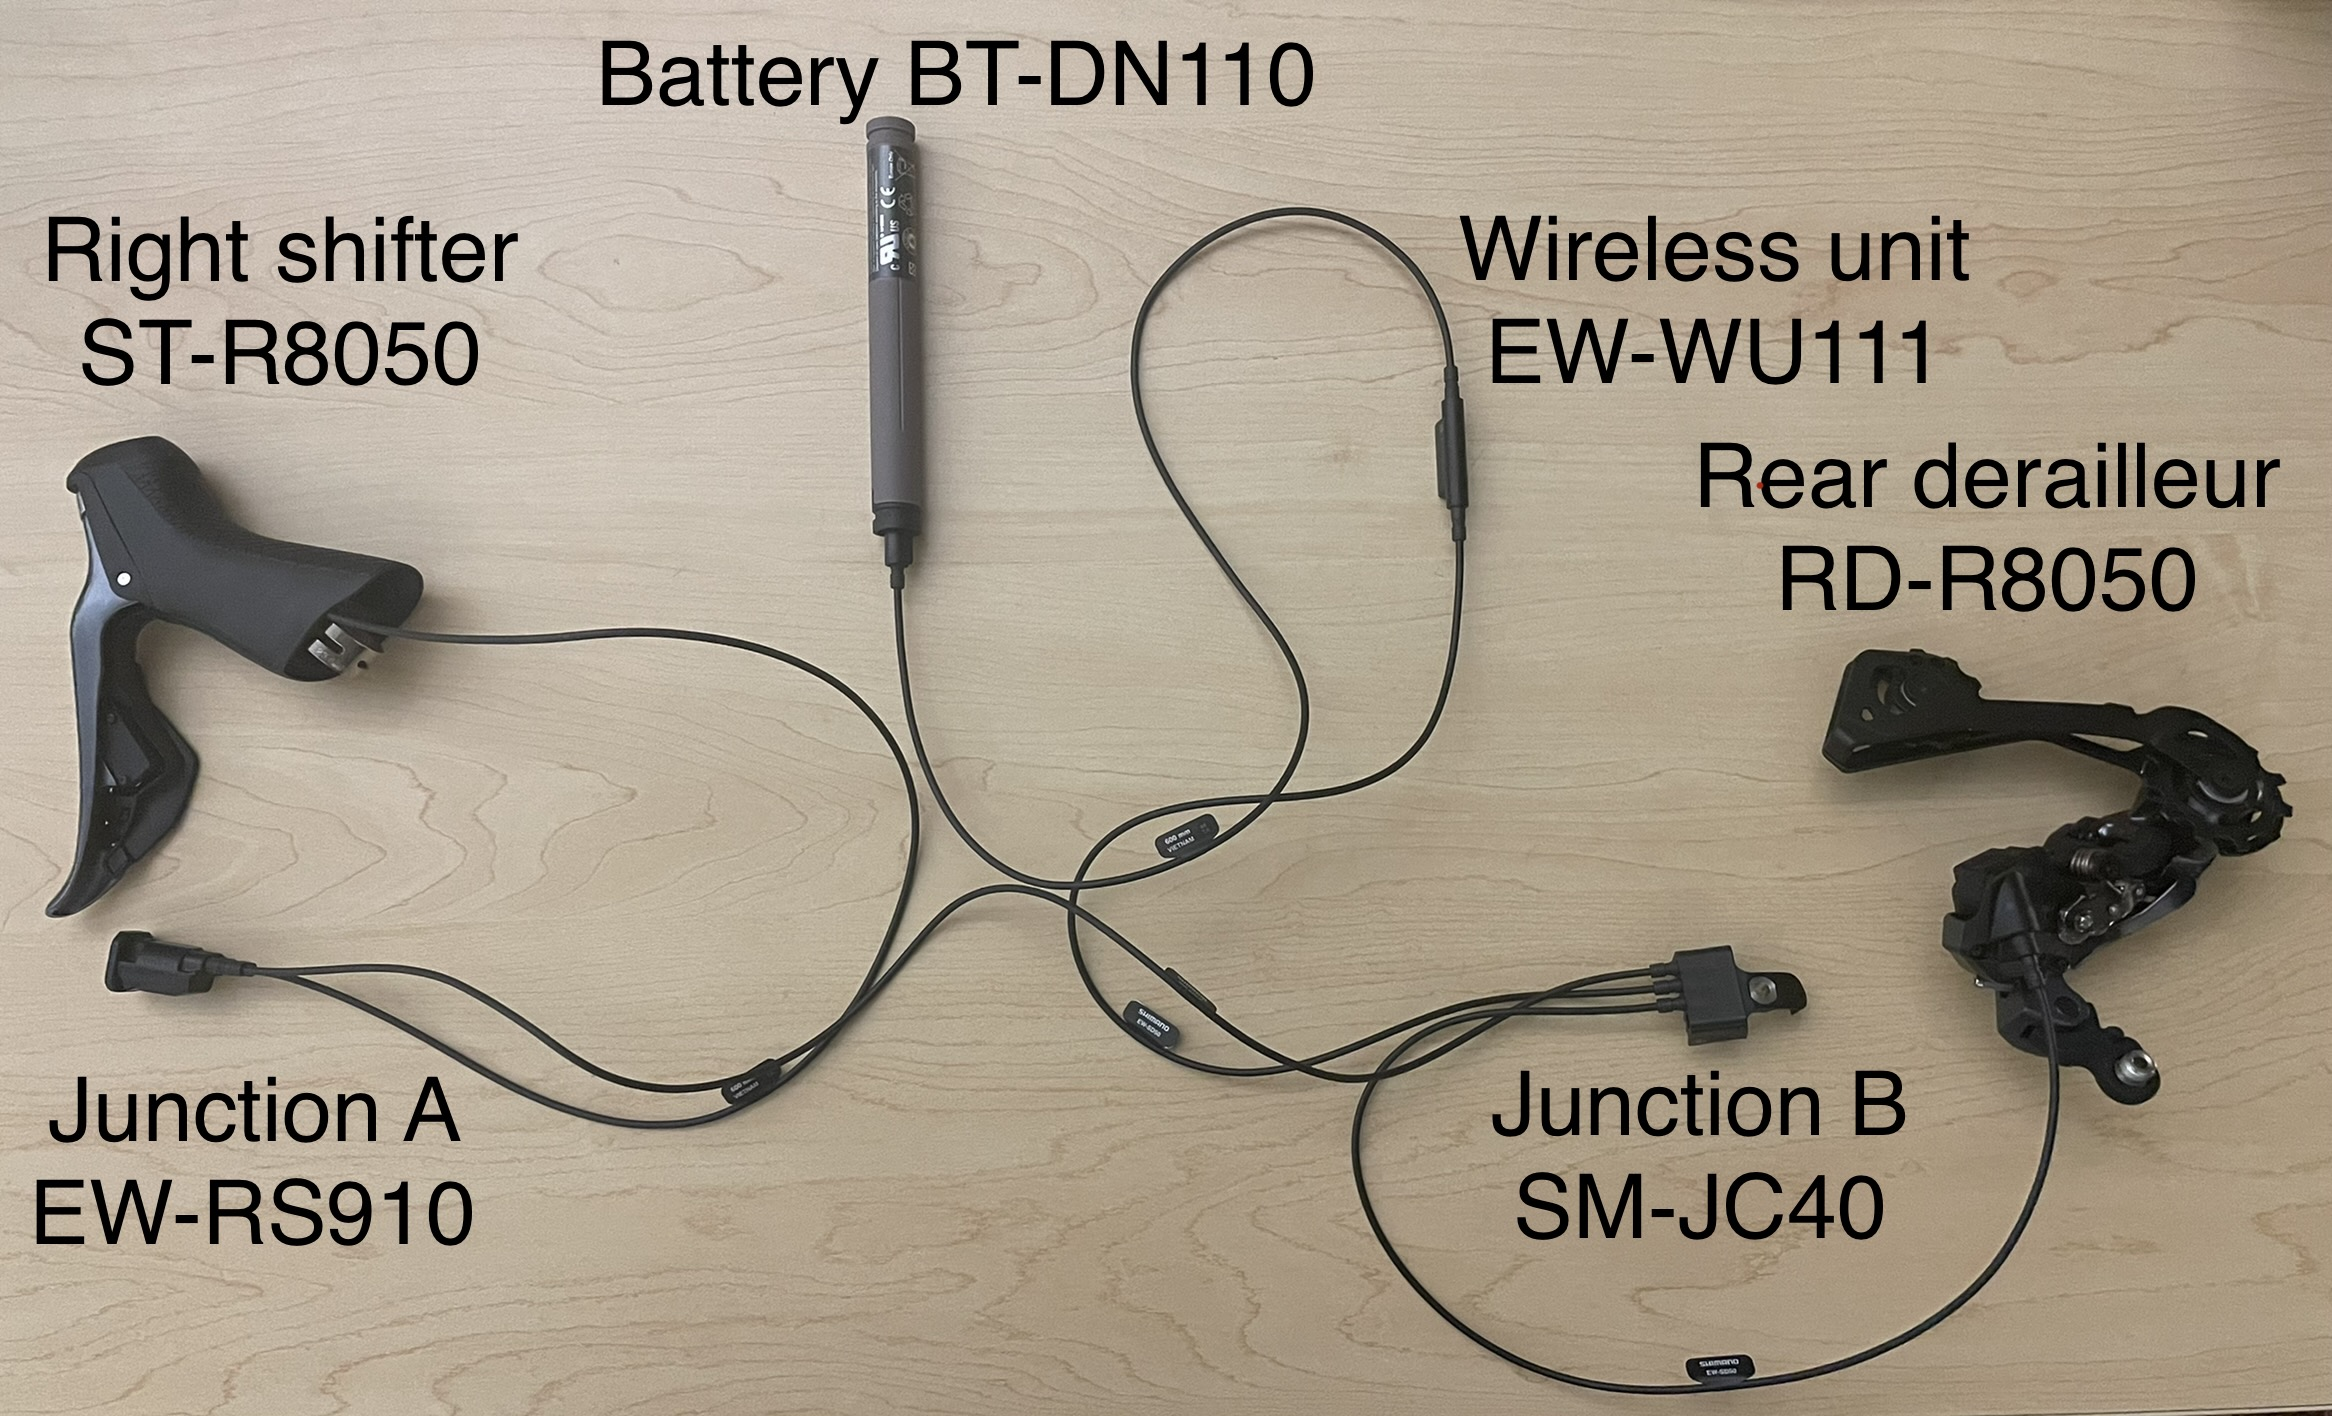
\includegraphics[width=0.4\textwidth]{images/IMG_5264_Di2.jpg}
    \label{fig:Di2Setup}
  \end{center}
  \caption{The battery sits inside the seat post while the rear derailleur sits on the back wheel. The junctions sit at mount points in the frame/handlebar, and the wireless unit floats freely in the frame}
\end{figure}


\subsection{SRAM Force eTap AXS}
The SRAM Force eTap AXS \cite{etap} is marketed toward professional, competitive bikers, and is priced the most premium out of all of our components. It works completely wirelessly like the Archer Components D1X meaning there is no need for physical wire between the derailleur and the shifters. The SRAM is also the only one in our lineup that uses a proprietary protocol. The derailleur and the shifter communicate using the in-house AIREA protocol that operates within the 2.475Ghz frequency range. During a press event of this products, SRAM claims that  the protocol uses 128-bit rolling encryption and the system is "more secure than any cash machine" \cite{phillips2015SRAM}. The system also provides Bluetooth for connecting to a smartphone and ANT+ to send information to a bicycle computer.

To set up the SRAM system, the biker will have to click a button on the derailleur to enter pairing mode and then click the buttons on both shifters consecutively to finish the pairing process. To connect to a mobile phone, the biker will start an app on their phone, select their SRAM system, and long-press a button on the derailleur to authorize. Note that the app provides ways to remap each shifter to different operations (gear up, gear down), but the user is not able to shift the gear directly in the app.




\section{Security Analysis}



\subsection{Threat Model \& Goal}
We want to protect the safety of the bikers using electronic shifters as sudden shifting when unintended may cause harm. We assume a scenario where bikers are joined with some malicious actors in a large-scale biking competition. In this scenario, we assume the adversary has access to the type of shifter the victim is using. The adversary can also be in close proximity with the victim before or during the competition, as a result, they can send arbitrary radio signals to the victim. We further assume the adversary can have a very short period of physical access with the victim's bike before the competition, such as when the victim is going to a restroom.

We define a successful attack as making a victim's bike shift to an unintended gear during competition. We will also define a successful attack as making a victims bike be unable to respond to legitimate shifting commands during competition. We assume all competitors will do a quick test ride before the competition and don't consider denial of service before the competition as a successful attack since this does not introduce safety risks to the riders. For that reason, simple attacks such as cutting the victim's breaking cable or poking a hole in the victim's tire will be trivially easy to spot during the test ride and thus won't qualify as a successful attack.


\subsection{Bluetooth Pairing Weakness}
\begin{table}[]
  \begin{tabular}{|l|l|l|l|}
    \hline
            & \begin{tabular}[c]{@{}l@{}}Pairing \\ authentication\\ method\end{tabular} & \begin{tabular}[c]{@{}l@{}}Direct shift\\ from app\end{tabular} & \begin{tabular}[c]{@{}l@{}}Configure harmful\\ setting from\\ app\end{tabular} \\ \hline
    Archer  & None                          & Yes                           & Yes                           \\ \hline
    Shimano & 6 Digit Pin                   & Yes                           & Yes                           \\ \hline
    SRAM    & Button                        & No                            & Yes                           \\ \hline
  \end{tabular}
  \caption{Component Bluetooth pairing authentication methods and app capabilities}
  \label{tab:btauth}
\end{table}

All of our components provide Bluetooth connectivity and have companion mobile applications, so the user can configure or shift from their mobile phone. Like all Bluetooth products, a pairing process must be done before the user can interact with their device. Preventing unintended users from connecting is more important in biking shifters than traditional Bluetooth devices since a sudden change of gear when the biker is climbing or performing stunts can cause injuries to the riders. In addition, changes made to the gear settings from mobile applications aren't visible outside of the application. Our line up of components employ various degrees of authentication to prevent this from happenning. Table \ref{tab:btauth} summarize the components' authentication methods and their mobile apps' capabilities.

\paragraph{Archer D1X}
The Archer D1X groupset relies on the Bluetooth communication protocol for shifter/shifting-box communication along with communication with the mobile application. Once the shifting box is powered on anybody with the Archer mobile application can pair with it. There are no pairing authentication steps and this lack of validation means that those other than the legitimate owner can connect. Once an adversary has paired with the shifting box they can create custom gear-switch settings that would be harmful to the user. An adversary could swap the higher and lower gear switch buttons causing the cyclist to experience unexpected dangerous behavior. Gear setting changes made through the application are invisible to the cyclist and there is no mechanism of alerting the owner of such changes. The Bluetooth protocol only allows for one active device at a time meaning that only one device can be connected to the shifting box at a time.

\paragraph{Shimano}
Shimano has one of the most robust pairing systems of the tested gear sets. Although it defaults to no password, users can add up to a 6 digit password which prevents unauthorized users from logging on, and failed sign on attempts require a restart of the device, preventing brute force attacks or repeated sign on attempts from malicious users. Although this will deny Bluetooth service to the owner until they restart, they are still able to shift the bike using the shifter even after the Bluetooth users get locked out.

It also features updatable firmware through the app, where it first downloads the firmware onto the app, and then uploads it to the device. Firmware can be updated indidvidually for each device. Although we didn't test firmware attacks, this suggests it should be possible to spoof the source upload your own firmware onto the device.

\paragraph{SRAM}
The SRAM uses a more traditional pairing mechanism where the app will prompt the user to physically press a button on the derailleur to authorize a connection. The system can also only pair with one smartphone at a time, therefore, when another device wants to connect, a physical button press is required even if that device had paired with the system before. While this is the industry standard of such Bluetooth pairing process, several key differences make the solution not ideal for an electronic shifter.

\begin{itemize}
  \item \textbf{Highly possible to expose to an attacker} Unlike some Bluetooth personal belongings, such as a wireless headset, where the owner is expected to be always in possession of the device, bikes can be parked in a public space. Since the SRAM's pairing button is exposed as shown in Figure 2, the attacker will be able to pair with the bike in very a short period.
  \item \textbf{Not immediately noticable} Most Bluetooth devices use Bluetooth for their primary function. If the authorized device changes, the device owner will be locked out and immediately initiate a re-pair process, rendering the attacker’s device useless. However, in the case of an electronic shifter, the shifter is fully functional without any Bluetooth connection. Therefore, it will be very easy to overlook during a pre-ride checking and the attacker can choose a most dangerous time to send malicious command to the shifter.
\end{itemize}

\begin{figure}[ht]
  \begin{center}
    \centering
    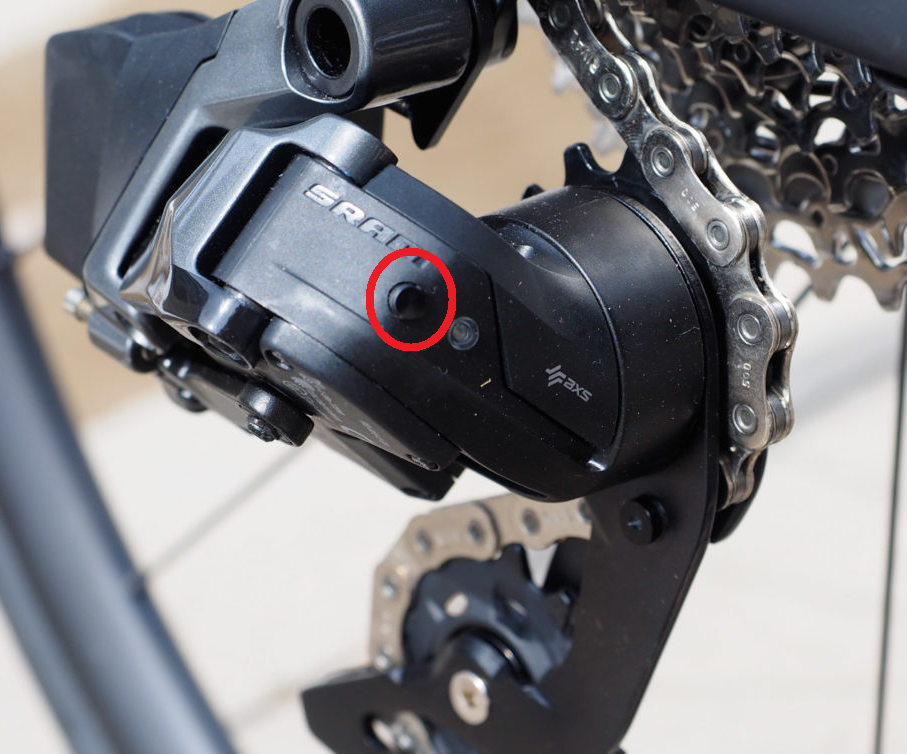
\includegraphics[width=130pt]{images/SRAMbtn.png}
    \label{fig:srambtn}
  \end{center}
  \caption{Exposed SRAM pairing button \cite{james_sram_2021}}
\end{figure}

Even though SRAM's app does not provide direct shifting capabilities, they also provide a way to swap the higher and lower gear switch, the adversary can wait for the exact moment to swap the switch thus poses threat to the rider. Furthermore, the system will not actively alert the owner that a pairing event had happened. The only way for the owner to notice is when they want to configure their bike as the app will prompt the user to re-pair to the bike. Even then, the user might not understand that their bike had been paired with other devices and not implement any safety measure.

\subsection{Archer Packet Examination}

Using an Ubertooth One we were able to capture and examine the pairing packets between the mobile application and the shifting box as well as the packets sent by the hand shifter to the shifting box. After the initial pairing process, the BLE packets become encrypted and the data in the packets is unreadable.

During our examination of the mobile applications sent packets we were hindered by the various security measures that Apple has implemented in its Bluetooth protocols \cite{appleblesecurity}. This includes spoofing the MAC address and changing it periodically making it difficult to discern which packets are meant for the Archer D1X shifter.

While we did not execute a DOS attack on either Archer component we can assume that it would be successful since prior research has shown success against all devices when large L2CAP packets are flooded \cite{bluesmack}. The only mitigations that currently exist against this attack are disabling Bluetooth when not in use and setting your device to non-discoverable mode. However, using the Ubertooth we can find the devices MAC when it is operating in non-discoverable mode.

\subsection{Shimano Packet Examination}

Using an Ubertooth One we were able to examine the packets sent from the mobile application to the Shimano groupset (which was given the device name EWWU111). The packets that we analyzed initiated a master/slave connection and began encryption upon sharing certain cryptographic keys (Random Number, Diversifier, Initialization Vector) in-line with the BLE-Legacy security protocol. After the encryption begins, we are no longer able to discern any information from the packets including the user provided pairing pin. We also had similar issues with Apple’s Bluetooth security protocols as described in Section 5.3 above.

We attempted to break the packet encryption using a tool called Crackle \cite{crackle}. Crackle exploits a design flaw in the Bluetooth pairing process allowing an attacker to brute force a temporary key relatively quickly using the packets found while listening to legitimate pairing transmissions. Since the Shimano device uses the legacy pairing (and not LE Secure Connections, introduced in Bluetooth 4.2) it should be suseptible to the attack as long as we have the minimum required three packets: LL\_ENC\_REQ, LL\_ENC\_RSP, and LL\_START\_ENC\_REQ.

\begin{figure}[ht]
  \begin{center}
    \centering
    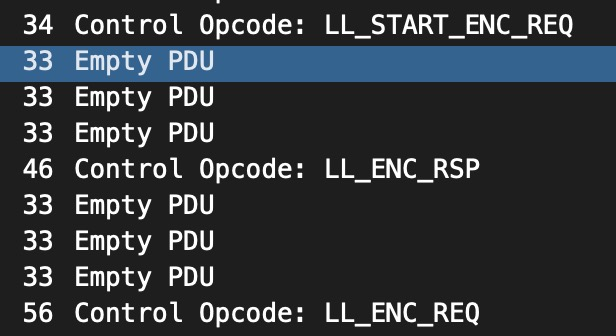
\includegraphics[width=230pt]{images/shimano-packets.jpeg}
    \label{fig:Replay}
  \end{center}
  \caption{Here we can see each of the three required packets in our logs}
\end{figure}

To do this, we saved packet logs containing the mobile application and shifter pairing packets and attempted to run them through crackle. Crackle was unable to break the encryption due to two missing pieces of pairing data, specifically, the Mrand and Srand values. Although it appears we were able to capture all three of the packets required by Crackle, our inability to find the Mrand and Srand values suggests Shimano uses a custom formatting which prevents this attack from working as it stands. Ultimately we weren't able to brute force the temporary key, and this all suggests to us that the Shimano Di2 is one of the more secure electronic systems on the market.

\subsection{SRAM Replay Attack}

\begin{figure}[ht]
  \begin{center}
    \centering
    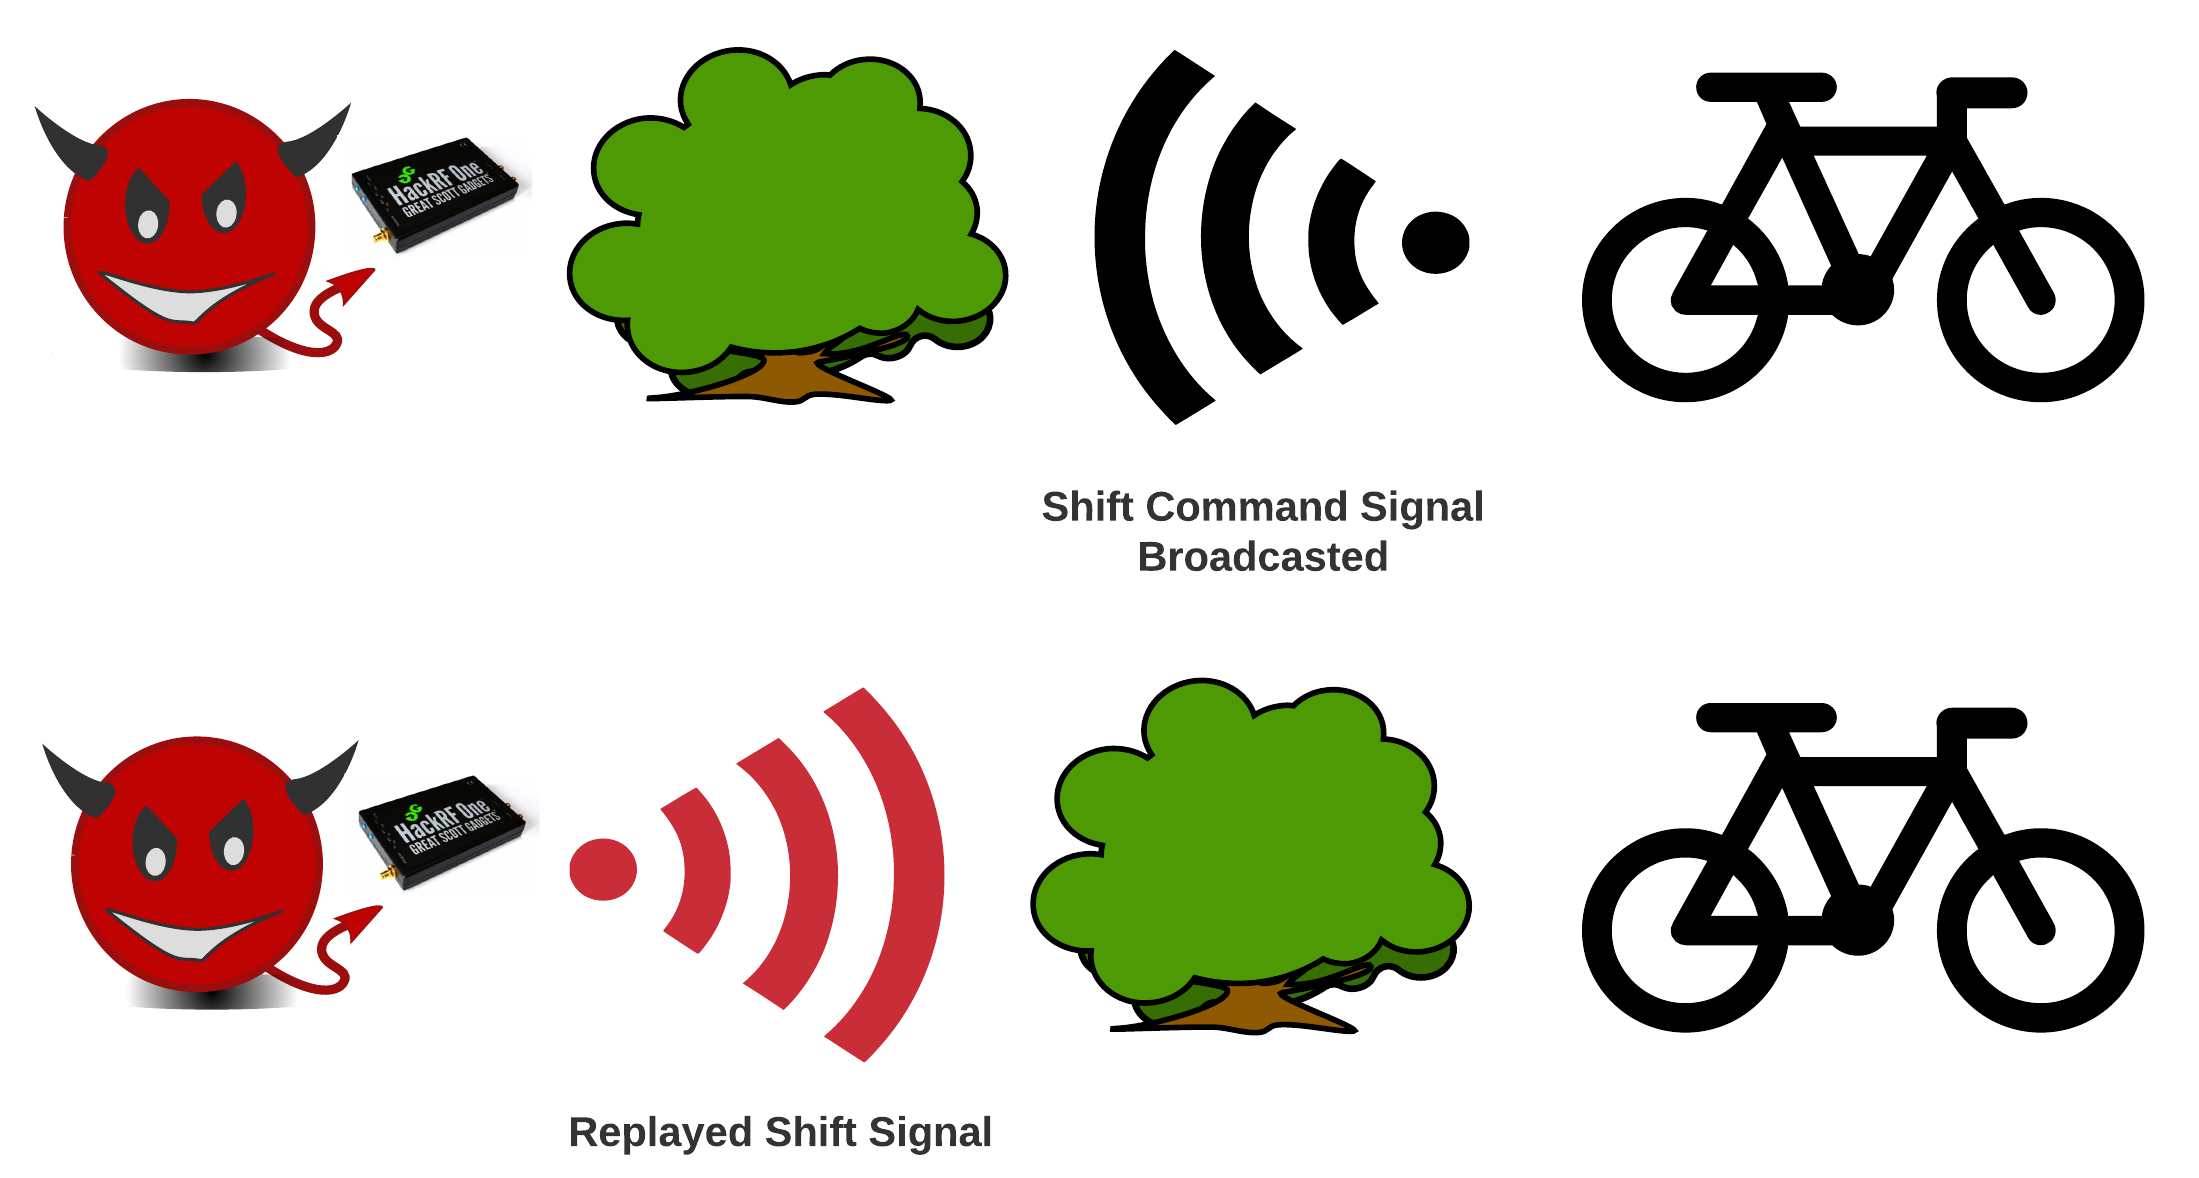
\includegraphics[width=230pt]{images/replay.png}
    \label{fig:Replay}
  \end{center}
  \caption{Visual depiction of an adversarial replay attack}
\end{figure}

\paragraph{SRAM ARIEA protocol} From public FCC data, we know that the SRAM system's operating frequency is around 2.475GHz with a bandwidth of 3MHz, therefore, we use an SDR and the Universal Radio Hacker software \cite{urh} to analyze the signals between the shifters and the derailleur. During the investigation, we reveal some facts about the protocol.
\begin{itemize}
  \item \textbf{The shifter emit signal} We find out that every time the shifter is pressed, it will emit a signal continuously for about 1.2 seconds.
  \item \textbf{No ACK-like signal from the derailleur} We verify this by turning off the derailleur and do not observe any significant difference in the captured signal compared with those captured with the derailleur on.
  \item \textbf{Two main types of packets} We discover that the left and right shifter emit different types of packets. The difference is so significant that it is observable from the waveform.
  \item \textbf{Effective range} While we do not measure the exact effective range of the system, we do find out that the derailleur responds even if the shifters and the derailleur are over 10 meters apart.
\end{itemize}

\paragraph{Replay vulnerability}
We further discover that recording a signal from a shifter and replaying it will cause the derailleur to act accordingly, though there are some restrictions. We can only replay the latest packets from each shifter (one per shifter). As soon as the user sends the same
type of signal (by pressing the same side of the shifter), the previously stored packet will be invalidated. We suspect that each shifter has its internal counter that the derailleur keep track of, so it can invalidate all previous packets after receiving a new one, but we are not able to confirm this.

\paragraph{Attack implementation} The ability to replay the latest packet still opens up a way to attack the system. Based on the aforementioned vulnerability, we designed an algorithm specifically to attack an SRAM system during competition. We set up the SDR in a way that it will continuously switch between receiver and sender mode. During the receiver mode, the SDR will capture signals from the air and detect if it contains an SRAM gearing signal. If it does, it stores the new signal. Then it will send the saved signal (either the newly captured one or something stored before) to the air, causing the victim's bike to shift unintendedly.

Since SRAM does not release their firmware let alone source code, we do not have a reliable way to detect whether a signal segment contains an SRAM shifting packet or not. Therefore, we use a simple SVM classifier to solve the problem. We prerecorded several SRAM gearing signal segments and trained the model along with white noise and signal from other 2.4Ghz devices. In the end, we can reach 100\% accuracy in a lab environment.

We setup the attack with a HackRF One SDR. Under the attack, when the victim shifts near the attacker, their derailleur will continuously shift to the highest or lowest, and even if the victim counter shift, they will find out that their system shift to the other extreme direction.
\begin{algorithm}
  \caption{SRAM replay attack algorithm}\label{alg:cap}
  \begin{algorithmic}[1]
    \State $saved \gets None$
    \While {$True$}
    \State Set up SDR in receiver mode
    \State $signal \gets$ get signal from SDR for 1 second
    \If{$signal\;match\;SRAM\;pattern$}
    \State $saved \gets signal$
    \State Setup SDR in sender mode
    \State Send $saved$
    \EndIf
    \EndWhile
  \end{algorithmic}
\end{algorithm}

\paragraph{Potential Optimization}
In the attack, if the victim happens to shift the same gear while the SDR is in sender mode,
subsequent attacks will fail. However, there are possible ways to optimize this attack.
\begin{itemize}
  \item \textbf{Use two SDRs one for receiving and one for sending.} Clearly, in this setting, the attacker will be able to notice the victim's signal while they are sending their malicious signal. However, the attacker's receiver will now be interfered by their sender, and special care needs to be done to avoid confusion.
  \item \textbf{Trim the saved data.} During investigation, we found out that while the signal from the shifter lasted over 1 second, 50ms worth of data is enough to cause the derailleur to act. Therefore, it is possible that we can trim the data so that the SDR can send the data and be in sender mode for just a little amount if time, greatly reducing the chance of missing the victim's signal.
\end{itemize}

\section{Recommendations}

Our first recommendation is the implementation of passcodes/PINS for pairing with smartphones. The Shimano Di2 implemented a 6 digit PIN for pairing that we found to be an effective measure for preventing basic attacks such as the one presented for the Archer in Section 5.2. While previous research by Shaked and Wool~ \cite{bluepin} has demonstrated that these PIN’s are easily crackable they present a first line of defense and implementations such as the Shimano’s require the attacker to manually restart the pairing process upon incorrect entry. Thus, we recommend that all connections to the shifters require a PIN and have a mechanism for temporarily locking out devices after incorrect entry.

Our second recommendation is the implementation of timestamps in shifting communication packets to prevent replay attacks such as the one demonstrated in 5. The inclusion of a timestamp in every packet would allow the systems to detect when a packet has been replayed later in time. Another possible approach would be the creation of session keys between the shifter and shifting box. These session keys would be generated every packet and a subsequent replay would be denied. Interestingly, the SRAM groupset creates a similar encryption code but only utilizes it to prevent the mixing of shifting signals from other bikes with the same groupset~ \cite{etapsecure}.


\section{Conclusions}

The shifters that we examined represent the forefront of wireless shifting in bicycles. As the field matures and consumer adoption increases we can expect security to be a larger concern.
In our paper, we presented a novel threat model that focuses on remote attacks that pose a direct threat to the user through unexpected shifting. In accordance with our threat model, we present several Bluetooth pairing vulnerabilities along with a replay attack on the SRAM groupset. We also discuss potential countermeasures to these vulnerabilities such as pairing PINS and session keys/timestamps for packets. Our findings represent the first analysis of the security landscape of wireless shifting in bicycles.


\section{Future Work}

The security landscape of wireless shifters remains largely unstudied and there are several specific areas that we would like to study further. Firstly, we would like to examine the firmware of the shifters for specific vulnerabilities. We would also like to the examine the security of firmware updates and see whether an adversary could load malicious code into the shifter. While we did examine the shifting packets, we would like to do further analysis. Specifically, we would like to spend more time configuring crackle and testing it against different logs. We would also like to attempt MITM and replay attacks with the packets. We would also like to configure a phone that doesn’t have Bluetooth security protocols such as those implemented by Apple. Lastly, we would like to attempt to hack Shimano’s new wireless shifting groupset~ \cite{newshimano}. While the one that we analyzed could connect to a mobile application for configuration the new groupset will have wireless communication between the shifter and derailleur. This increased attack surface opens up the possibility of a replay attack such as the SRAM one being possible.

  {\normalsize \bibliographystyle{acm}
    \bibliography{references}}


\section{Appendix}
During the research we used the following firmware versions:
\begin{itemize}
  \item Archer D1X Phone App 1.8, No Visible Firmware version
  \item Shimano E-TUBE Phone App 5.0.2
  \item Shimano Di2 RD-R8050-GS 3.3.0
  \item Shimano Di2 ST-R8050 3.2.1
  \item Shimano Di2 EW-RS910 3.1.2
  \item Shimano Di2 EW-WU111 3.1.2
  \item Shimano Di2 BT-DN110 4.4.4
  \item SRAM eTAP Phone App 2.0.9, Firmware Version 2.7.6
\end{itemize}
\section{Group Contributions}

Most of the work and attack planning was done in group meetings, although we were still able to split a lot of the work up by component. Together we got the Archer, Di2, and SRAM working, and did some of the initial replay attacks against the SRAM together. Cody wrote the code and finished testing the SRAM replay attack and examine its bluetooth pairing properties. Since the Shimano and Archer both relied on Bluetooth, Tolga and Thomas worked together to test the Shimano Di2 and Archer Components D1x shifters and examine their Bluetooth protocols. We all took part in writing the final paper and slide presentation.

% \theendnotes

\end{document}


% Some embedded literal typset code might 
% look like the following :

% {\tt \small
% \begin{verbatim}
% int wrap_fact(ClientData clientData,
%               Tcl_Interp *interp,
%               int argc, char *argv[]) {
%     int result;
%     int arg0;
%     if (argc != 2) {
%         interp->result = "wrong # args";
%         return TCL_ERROR;
%     }
%     arg0 = atoi(argv[1]);
%     result = fact(arg0);
%     sprintf(interp->result,"%d",result);
%     return TCL_OK;
% }
% \end{verbatim}
% }

% you can also use the wonderful epsfig package...
% \begin{figure}[t]
% \begin{center}
% \begin{picture}(300,150)(0,200)
% \put(-15,-30){\special{psfile = images/piezospeaker.png hscale = 50 vscale = 50}}
% \end{picture}\\
% \end{center}
% \caption{Wonderful Flowchart}
% \end{figure}


% Example image
% \begin{figure}[ht]
% \begin{center}
% \centering
% \includegraphics[width=0.4\textwidth]{images/2msSig18.png}
%
% \label{fig:2msSignal}
% \end{center}
% \caption{Above is a signal generated with data, where each bit was transmitted over 2ms. This allowed us % to create high resolution bit maps where the bits are distinguishable from each other.}
% \end{figure}


% An example table if we need to display data
%
% \begin{table}[]
% \begin{tabular}{|l|l|r|}
% \hline
% \multicolumn{1}{|c|}{Action}        & Code   & Distance                      \\ \hline
% Right turn                          & 0b0001    &                               \\ \hline
% Left turn                           & 0b0010   &                               \\ \hline
% Change lane (right)                 & 0b0011   &                               \\ \hline
% Change lane (left)                  & 0b0100  &                               \\ \hline
% Merge (right)                       & 0b0101  &                               \\ \hline
% Merge (left)                        & 0b0110  &                               \\ \hline
% Offramp                             & 0b0111  & \multicolumn{1}{l|}{}         \\ \hline
% Temporarily change lanes (incident) & 0b1000 & \multicolumn{1}{l|}{}         \\ \hline
% Speed (speeding up)                 & 0b1001 & \multicolumn{1}{l|}{Not used} \\ \hline
% Speed (slowing down)                & 0b1010 & \multicolumn{1}{l|}{Not used} \\ \hline
% \end{tabular}
% \end{table}



% Itemized list example
%
% \begin{itemize}
% \item Example itemized list
% \item Item 2
% \end{itemize}


% Equation Example:
% 
% $$ f = f_{0} \frac{c \pm v_{r}}{c \pm v_{t}} $$


% Example Code
%
% {\tt \small
% \begin{verbatim}

% generateSignal(dataSet)
%     lf = rand_low_freq
%     hf = rand_low_freq + frequency_shift

%     bits = [1,0,1,0,0,1,dataSet]
%     freqs = ones(length(bits)) .* lf

%     % assign 1 bits to high frequency
%     for 1 = 1:length(bits)
%         if bits(i) == 1
%             freqs(i) = hf
%         end
%     end

%     % add frequencies to signal
%     for i = 1:length(packet)
%         t = 0:1/fs:bit_duration;
%         f = sin(2*pi*packet(i).*t + phase);

%         % update phase
%         phase = phase + 2*pi*packet(i)*bit_duration;

%         % add in next position
%         ff(start_leg:end_leg) = f;
%     end
% end
% \end{verbatim}}
